\subsection{追従のためのフィードフォワード}

摩擦、不感帯、バックラッシュを補償しても、フィードバックだけで既知の速度や軌道を追う場合には一つの遅れが残る。フィードバックは、測定値が目標値からずれた後に操作量を増やす構造である。すでに分かっている目標速度、目標加速度、目標軌道の曲率、または測定済みの負荷外乱があるなら、それらを偏差が現れる前に操作量へ入れられる。この先回り入力がフィードフォワードである。

ここで扱うフィードフォワードは、フィードバックを置き換えるものではない。補償後の DC モータでも、名目慣性、粘性係数、トルク定数、車輪半径、路面状態は真値と完全には一致しない。したがって、既知の運動に必要な入力を先に入れ、残ったモデル誤差、初期値のずれ、未測定外乱、飽和の影響をフィードバックで戻す、という役割分担で使う。

\subsubsection{速度と加速度から作る DC モータの先回り電流}

前段までのカスケード制御では、電流ループが十分速い範囲で速度ループから見る入力を電流指令として扱った。摩擦補償後の速度軸を
\begin{equation}
  J\dot{\omega}+b\omega+\tau_f(\omega)+\tau_L=K_t i
  \label{eq:feedforward-motor-model}
\end{equation}
で表す。$\omega\,[\mathrm{rad/s}]$ は角速度、$i\,[\mathrm{A}]$ は電流、$J\,[\mathrm{kg\,m^2}]$ は慣性、$b\,[\mathrm{N\,m\,s/rad}]$ は粘性係数、$K_t\,[\mathrm{N\,m/A}]$ はトルク定数、$\tau_f$ は摩擦トルク、$\tau_L$ は負荷トルクである。前節の摩擦補償で $\tau_f$ の主要成分を入力側へ入れた後でも、目標角速度 $\omega_r(t)$ を急に変えると、加速に必要なトルク $J\dot{\omega}_r$ は偏差が出る前に必要になる。

名目値 $J_n,b_n,K_{t,n}$ と、必要なら目標速度上で評価した摩擦補償 $\hat{\tau}_{f,r}$ を使うと、速度・加速度フィードフォワード電流は
\begin{equation}
  i_{ff}
  =
  \frac{
    J_n\dot{\omega}_r
    +b_n\omega_r
    +\hat{\tau}_{f,r}
    +\tau_{L,m}
  }{K_{t,n}}
  \label{eq:speed-acceleration-feedforward}
\end{equation}
である。$\tau_{L,m}$ は測定された負荷トルクであり、測れない場合は 0 とおく。加速度項 $J_n\dot{\omega}_r/K_{t,n}$ は速度を変えるための電流、粘性項 $b_n\omega_r/K_{t,n}$ はその速度を保つための電流、負荷項 $\tau_{L,m}/K_{t,n}$ は測定済みの外乱を相殺する電流である。

実際の電流指令は、フィードフォワードだけでなく速度偏差も使って
\begin{align}
  e_\omega&=\omega_r-\omega,\\
  i_c&=i_{ff}+K_P e_\omega+K_I\int e_\omega\,dt,\\
  i&=\operatorname{sat}_{[-I_{\max},I_{\max}]}(i_c)
  \label{eq:feedforward-feedback-current}
\end{align}
とする。$K_P$ の単位は $\mathrm{A/(rad/s)}$、$K_I$ の単位は $\mathrm{A/rad}$ である。フィードフォワードが正しければ $e_\omega$ は小さくなり、フィードバックは大きな追従入力ではなく補正入力として働く。名目値がずれていれば、式 \eqref{eq:feedforward-feedback-current} の比例・積分項が残差を修正する。

\begin{figure}[tbp]
\centering
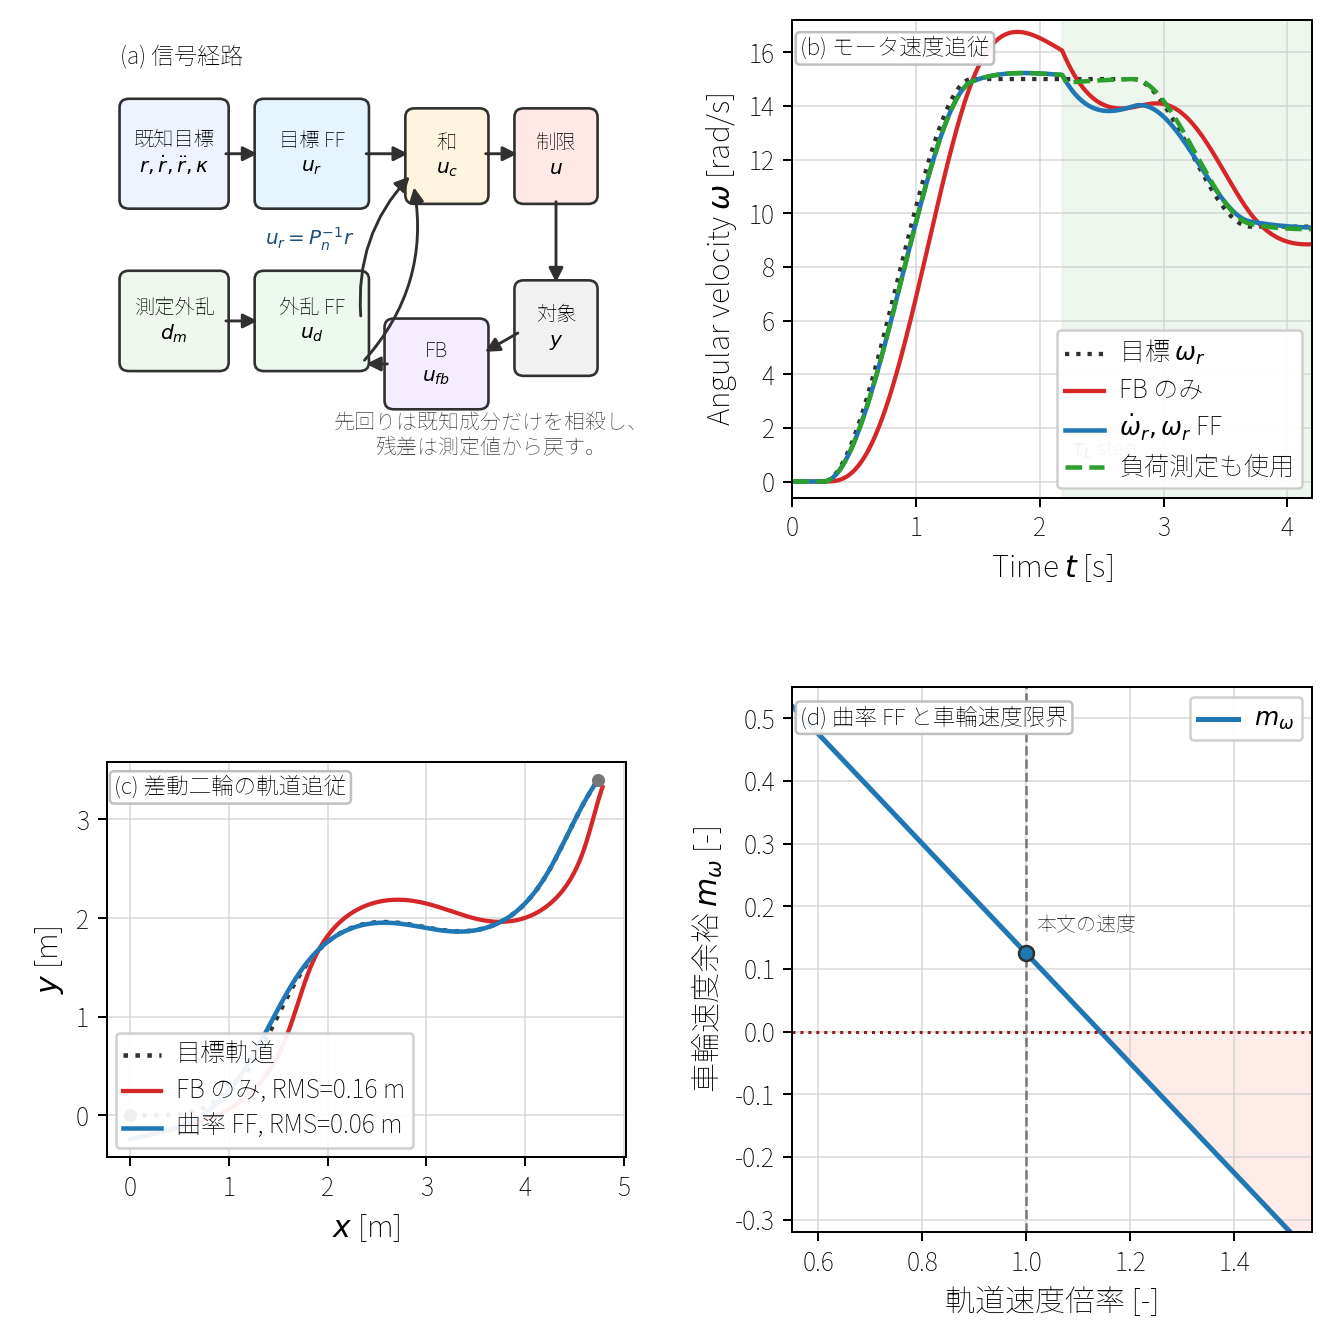
\includegraphics[width=0.98\linewidth,bb=0 0 1332 1332]{figures/feedforward_tracking_examples.png}
\caption{速度・加速度フィードフォワード、曲率フィードフォワード、測定外乱補償の役割。上段左は、既知目標と測定外乱から先回り入力を作り、残差をフィードバックで戻す信号経路である。上段右は DC モータ速度追従で、$\dot{\omega}_r$ と $\omega_r$ から作る電流を加えると立上り遅れが減り、負荷トルク測定 $\tau_{L,m}$ も使うと負荷投入後の速度低下がさらに小さくなる。下段左は差動二輪ロボットの軌道追従で、曲率フィードフォワードを入れると曲がり始めの横偏差が減る。下段右は軌道速度倍率を上げたときの車輪速度余裕 $m_\omega$ で、曲率が大きい軌道ほど外側車輪の上限が追従可能性を決める。}
\label{fig:feedforward-tracking-examples}
\end{figure}

\wfig{feedforward-tracking-examples} の上段右では、速度目標を滑らかに上げた後、$t=2.18\,\mathrm{s}$ で負荷トルクを加えている。フィードバックだけの場合は、目標が動き出してから速度偏差が増え、その偏差によって電流が増えるため、立上りで遅れる。式 \eqref{eq:speed-acceleration-feedforward} の速度・加速度項を入れると、加速に必要な電流が最初から出るので、追従誤差は小さくなる。さらに負荷トルクが測定できる場合は、$\tau_{L,m}/K_{t,n}$ を同じ電流指令に足すことで、負荷投入直後の速度低下を小さくできる。ただし図の緑線にも小さな残差がある。測定遅れ、名目値誤差、電流制限、摩擦補償の残りがあるため、測定外乱補償を入れてもフィードバックは必要である。

\subsubsection{差動二輪ロボットの曲率フィードフォワード}

速度フィードフォワードは一軸モータだけの考え方ではない。差動二輪ロボットでは、追いたい軌道の中心速度と曲率が分かっていれば、左右車輪がどの速度で回るべきかを偏差が出る前に計算できる。車輪半径を $r_w\,[\mathrm{m}]$、左右車輪間隔を $B\,[\mathrm{m}]$、車体中心の目標並進速度を $v_r(t)\,[\mathrm{m/s}]$、目標曲率を $\kappa_r(t)\,[1/\mathrm{m}]$ とする。曲率は弧長 $s$ に対する姿勢角 $\psi$ の変化率
\begin{equation}
  \kappa_r=\frac{d\psi_r}{ds}
  \label{eq:path-curvature-definition}
\end{equation}
であり、時間微分では
\begin{equation}
  \dot{\psi}_r
  =
  \frac{d\psi_r}{ds}\frac{ds}{dt}
  =
  \kappa_r v_r
  \label{eq:yaw-rate-curvature}
\end{equation}
となる。したがって、左右車輪の目標角速度は
\begin{align}
  \omega_{\mathrm{R},ff}
  &=
  \frac{
    v_r+\frac{B}{2}\dot{\psi}_r
  }{r_w}
  =
  \frac{
    v_r\left(1+\frac{B}{2}\kappa_r\right)
  }{r_w},\\
  \omega_{\mathrm{L},ff}
  &=
  \frac{
    v_r-\frac{B}{2}\dot{\psi}_r
  }{r_w}
  =
  \frac{
    v_r\left(1-\frac{B}{2}\kappa_r\right)
  }{r_w}.
  \label{eq:differential-drive-curvature-feedforward}
\end{align}
直線では $\kappa_r=0$ なので左右は同じ速度になる。左へ曲がる正の曲率では、右車輪が外側を通るため $\omega_{\mathrm{R},ff}$ が大きくなり、左車輪は小さくなる。

軌道追従では、式 \eqref{eq:differential-drive-curvature-feedforward} をそのまま出すだけでは初期位置ずれを戻せない。そこで、参照姿勢 $\psi_r$ の座標系で位置誤差を
\begin{align}
  e_x&=\cos\psi_r(x_r-x)+\sin\psi_r(y_r-y),\\
  e_y&=-\sin\psi_r(x_r-x)+\cos\psi_r(y_r-y),\\
  e_\psi&=\operatorname{wrap}(\psi_r-\psi)
  \label{eq:trajectory-error-frame}
\end{align}
と定義する。$e_x$ は軌道方向、$e_y$ は横方向、$e_\psi$ は向きの誤差である。簡単な追従則として
\begin{align}
  v_c&=v_r+k_xe_x,\\
  \dot{\psi}_c&=v_r\kappa_r+k_y e_y+k_\psi e_\psi
  \label{eq:curvature-feedforward-feedback-law}
\end{align}
を使う。第二式の先頭 $v_r\kappa_r$ が曲率フィードフォワードであり、残りの $k_y e_y+k_\psi e_\psi$ が横偏差と姿勢偏差を戻すフィードバックである。曲率項を抜くと、ロボットは曲がるべき場所に来ても直進を続け、横偏差または姿勢偏差が生じてから初めて旋回する。曲率項を入れると、目標軌道が曲がり始める時点で左右車輪速度が分かれ、フィードバックは初期ずれとモデル誤差の補正に回る。

\wfig{feedforward-tracking-examples} の下段左は、同じ初期ずれから始めた差動二輪ロボットの比較である。赤線のフィードバックのみでは、曲率が変わるたびに横偏差が先に発生し、その後に向きが戻る。青線の曲率フィードフォワードでは、式 \eqref{eq:differential-drive-curvature-feedforward} により外側車輪と内側車輪の速度差が先に作られるため、同じフィードバックゲインでも軌道中心に近いまま曲がれる。

\subsubsection{逆モデルフィードフォワードの範囲と限界}

速度・加速度項も曲率項も、広い意味では「望む出力から必要入力を逆に計算する」処理である。線形対象を
\begin{equation}
  y=P(s)u+P_d(s)d
  \label{eq:inverse-model-feedforward-plant}
\end{equation}
と書き、名目モデルを $P_n(s),P_{d,n}(s)$ とする。目標値 $r$ に対して名目上 $y=r$ を満たしたいなら、形式的には
\begin{equation}
  u_r=P_n^{-1}(s)r
  \label{eq:nominal-inverse-reference-feedforward}
\end{equation}
である。測定外乱 $d_m$ がある場合は、外乱から出力までの影響を打ち消すように
\begin{equation}
  u_d=-P_n^{-1}(s)P_{d,n}(s)d_m
  \label{eq:measured-disturbance-feedforward}
\end{equation}
を加える。モータ負荷トルクの例では、$d_m=\tau_{L,m}$、$u_d=\tau_{L,m}/K_{t,n}$ であり、式 \eqref{eq:speed-acceleration-feedforward} の負荷項に対応する。

しかし、式 \eqref{eq:nominal-inverse-reference-feedforward} と式 \eqref{eq:measured-disturbance-feedforward} はそのまま使えるとは限らない。第一に、$P_n^{-1}$ がプロパーで安定でなければ、微分を過剰に要求したり、右半平面零点やむだ時間を不安定な逆として反転したりする。第二に、モデルが合っていても入力制限がある。\wfig{feedforward-tracking-examples} の下段右では、車輪速度余裕を
\begin{equation}
  m_\omega
  =
  1-
  \frac{
    \max(|\omega_{\mathrm{L},c}|,|\omega_{\mathrm{R},c}|)
  }{\Omega_{\max}}
  \label{eq:wheel-speed-margin-feedforward}
\end{equation}
で評価している。$m_\omega>0$ なら左右車輪指令は上限 $\Omega_{\max}$ の内側にあり、$m_\omega<0$ なら曲率フィードフォワードが要求する車輪速度を実機が出せない。軌道速度倍率を上げると $v_r$ と $\dot{\psi}_r=v_r\kappa_r$ が同時に増えるため、外側車輪の余裕が先に消える。

第三に、測定外乱補償は測定できる成分だけを相殺する。負荷トルク計が遅れを持つ場合、床面の傾きや摩擦変化を測っていない場合、または外乱の作用点を名目モデルが誤っている場合、式 \eqref{eq:measured-disturbance-feedforward} の相殺は完全ではない。測定値にノイズがあると、外乱フィードフォワード自体が入力ノイズになることもある。

このため、実装上の構成は
\begin{equation}
  u
  =
  \operatorname{sat}
  \left(
    u_r+u_d+u_{fb}
  \right),
  \qquad
  u_{fb}=C(r-y)
  \label{eq:feedforward-feedback-implementation}
\end{equation}
である。$u_r$ は既知目標の先回り入力、$u_d$ は測定外乱の先回り補償、$u_{fb}$ は残差を戻す入力である。フィードフォワードを入れるほど、フィードバックが修正する誤差は小さくできるが、フィードバックをなくすと、初期ずれ、モデル誤差、未測定外乱、飽和後の入力不足を戻す経路がなくなる。したがって、ここでの結論は、フィードフォワードで「予測できる入力」を先に払い、フィードバックで「予測できなかった差」を測定から戻す、という分担である。この分担を信頼するためには、次に名目モデルがどの程度実機に合っているかを同定とモデル検証で評価する必要がある。
